To run a simulation, at least 4 files are needed :
\begin{itemize}
	\item The \cas for \courlis [Section \ref{cas_files}]
	\item The \xcas for \mascaret [Section \ref{cas_files}]
	\item The geometry file for \mascaret (\telfile{geometry.geo}) [Section \ref{geo_file}]
	\item The sediment layers file for \courlis (\telfile{geometry.geoC}) [Section \ref{geoC_file}]
\end{itemize}
Additional inputs can be used to specify liquid and solid boundary conditions or initial states. 

\section{The cas and xcas files}
\label{cas_files}
\subsection{Current set-up}
The \xcas containing \mascaret set up information can be adapted from \mascaret calculations or generated thanks to \fudaa (available at \url{www.opentelemac.org}). The reader can refer to the \mascaret guide for more information.

From a \mascaret file, the \courlis module is activated by modifying xml lines in the \xcas as described below :

\begin{figure}[htb!]
    \centering
    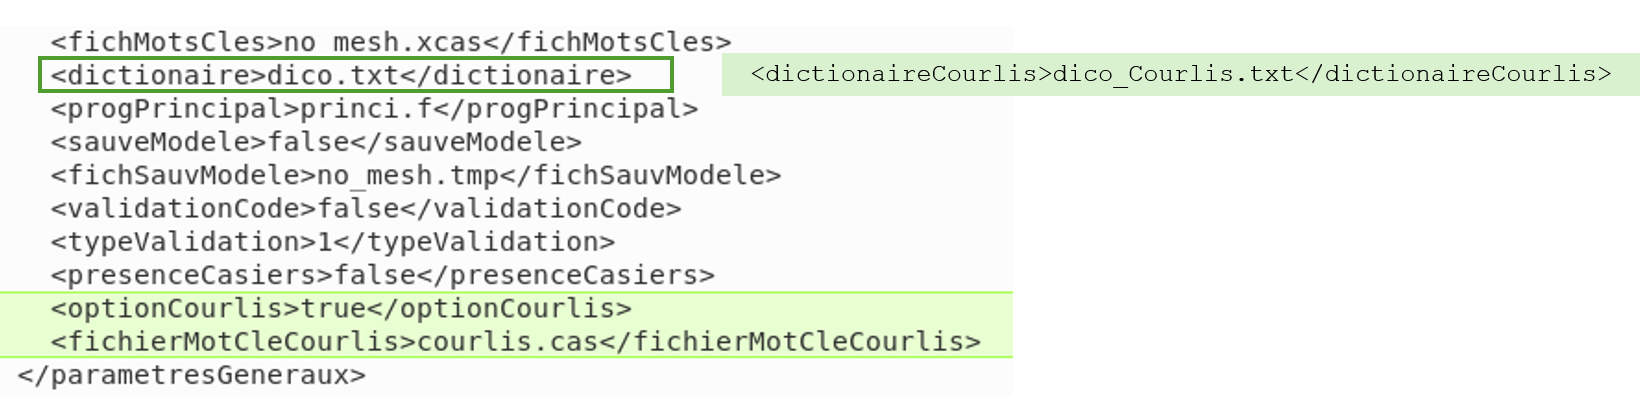
\includegraphics[width=0.9\textwidth]{./graphics/xcas_courlis.png}
    \caption{Changes in the \xcas to activate \courlis}
    \label{fig:xcas}
\end{figure}

First, the \courlis dictionary replaces the \mascaret one. Two lines are added to specify the activation of \courlis (\telkey{<optionCourlis>true</optionCourlis>}) and the name of the \courlis \cas (in this example called \telfile{courlis.cas}). 
These changes will call the \courlis routines with the parameters given in the corresponding \cas. \courlis can be shut off at any time by setting \telkey{<optionCourlis>false</optionCourlis>} resulting in a traditionnal \mascaret simulation. 

An example of an \xcas is given in Appendix \ref{app:xcas}. 

\begin{WarningBlock}{Warning}
	\fudaa provides an interface to generate \xcass but since \fudaa v7p2, the software is no longer supported. Consequently, 4 tags xml are missing from \xcass generated with \fudaa :
	\begin{itemize}
		\item	The \courlis dictionnary tag (Figure \ref{fig:xcas})
		\item 	The \courlis option tag (Figure \ref{fig:xcas})
		\item	The \courlis key file tag (Figure \ref{fig:xcas})
		\item 	The uncentered scheme option tag for the permanent kernel of \mascaret (Figure \ref{fig:xcas_decentrement})
	\end{itemize}
	If a \fortran error (\verb"At line 531 of file .../pretrait.f90") appears while running \mascaret with SARAP it may be that the recently developed option of uncentered scheme for this kernel has not been added to the \xcas.
\end{WarningBlock}

\begin{figure}[htb!]
    \centering
    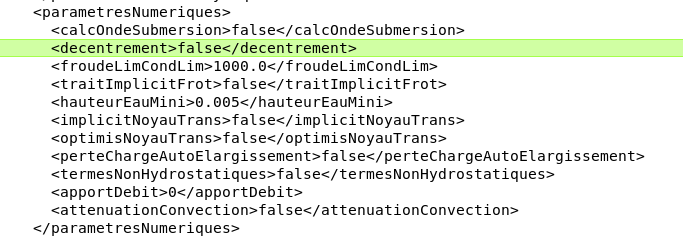
\includegraphics[width=0.8\textwidth]{./graphics/decentrement_xcas.png}
    \caption{Changes in the \xcas to add the uncentered option (set to \telkey{TRUE} to activate it)}
    \label{fig:xcas_decentrement}
\end{figure}

The \cas put in the \xcas controls \courlis parameters.
\courlis keywords, gathered in this file, are presented in the next sections.
An example is given in Appendix \ref{app:cas}. 

\subsection{Coming set-up}
Soon the code will only parse \xcass, one for \mascaret and one for \courlis, and no longer one \xcas for \mascaret and one \cas for \courlis. Nevertheless, thanks to \python script, the user will have the choice to launch the calculation with two \cass or two \xcass.

This improvement will make \mascaret parameters more readable and intuitive to facilitate its use.
\xcass can be converted to \cas via the command \\
\verb|manip_cas.py xcas2cas_1d <my_xcas_file.xcas> <output_cas_file.cas>|.

\begin{CommentBlock}{Warning}
	The keywords are not yet all translated in the dictionnary. So, in v8p3, this conversion will make a mixed english/french \cas !
\end{CommentBlock}

%%%%%%%%%%%%%%%%%%% GEOMETRY %%%%%%%%%%%%%%%%%%%%%
\section{Geometry and sediment layers}
\label{sedi_layers}

\subsection{The .geo file}
\label{geo_file}

The geometry file contains the initial bottom elevations of the reach, i.e. the initial elevation of the interface between the bottom and the water. 
Simple geometries can be generated thanks to \fudaa. Extraction of profiles from bathymetric measurements can be done thanks to \precourlis\footnote{In QGIS : \url{https://plugins.qgis.org/plugins/PreCourlis/} or GitHub : \url{https://github.com/msecher/PreCourlis}}.
While using \courlis, no mesh can be generated during simulation. That is why, unlike \mascaret, the cross-sections must be interpolated in pre-treatment.
If the space step of the geometry is not sufficient, interpolation can also be done with \precourlis.

\begin{CommentBlock}{Warning}
	It is recommended to avoid as much as possible vertical walls in geometry when using \courlis. Indeed, some approximations are done by \mascaret when lateral walls are vertical and hydraulics errors will be amplified by \courlis calculations. 
\end{CommentBlock}

\subsection{The .geoC file}
\label{geoC_file}

The \courlis geometry file contains the initial elevations of the different sediment interfaces. 

For each cross-section, the first column corresponds to the bottom layer as specified in the \telfile{geo file}. The next columns correspond to the different interfaces between sediment layers (as shown below). The last column corresponds to a non-erodable substratum (hard bottom). 
With the suspension module, two virtual layers are commonly set to represent sand and silt transport i.e. the initial width of these two layers is null. A third layer can be added to represent sediment already present in the initial step. This configuration corresponds to 4 interfaces in the \telfile{geoC file} as represented below
When modeling bedload, only one layer is useful and therefore 2 interfaces are given in the \telfile{geoC file} as represented below. 

\begin{figure}[htb!]
    \centering
    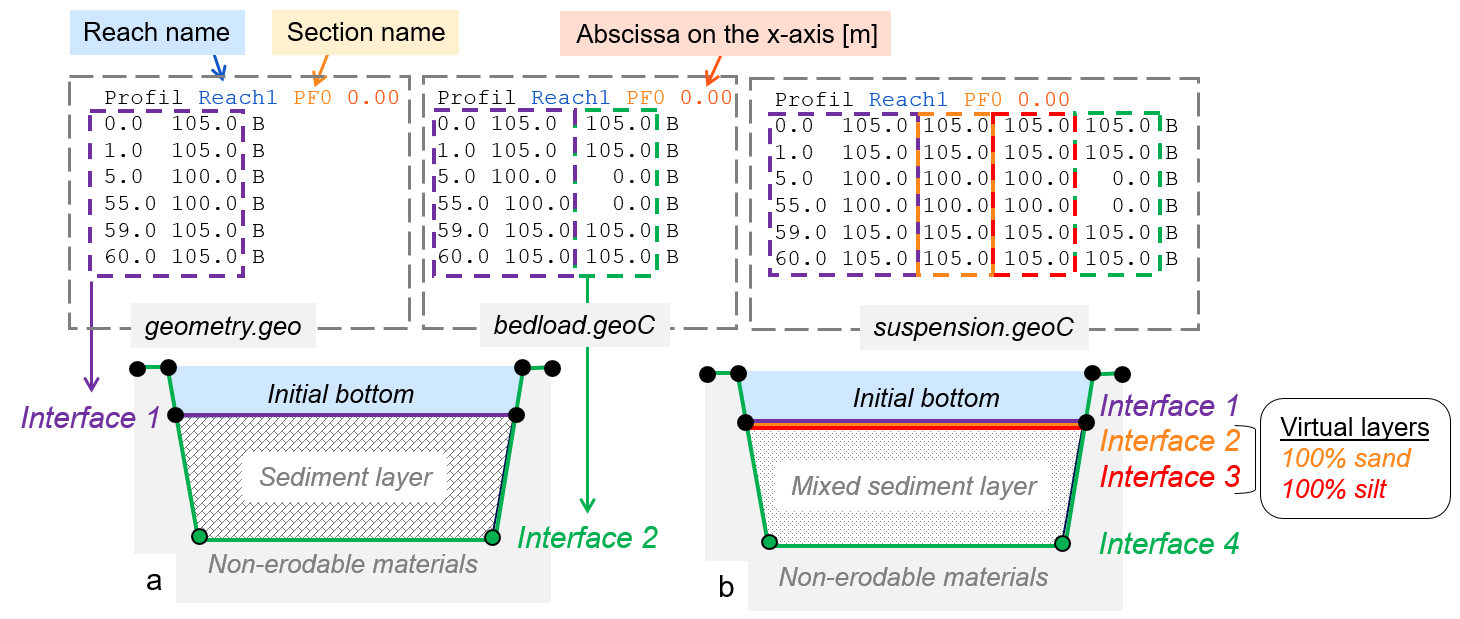
\includegraphics[width=\textwidth]{./graphics/geo_files.png}
    \caption{Examples of one cross-section in the \telfile{geo and geoC files} for (a) bedload and (b) suspension simulations}
    \label{fig:geo_files}
\end{figure}

\section{Optional inputs}
\label{optional_inputs}

Hydraulics boundary conditions are often written in an external file, for example \telfile{hydrograph.loi} at the upstream boundary and \telfile{elevation.loi} at the downstream boundary. Initial free surface elevations can also be given in an external file for example called \telfile{init.lig}. All external files names are specified in the \xcas. The reader can refer to the \mascaret guide for more information.\\

Similarly, sediment concentrations at boundaries can be given to \courlis from external files, for example \telfile{qs.loi}. The corresponding \telkey{LOI CONC X MODE D''ENTREE} keyword, with \telkey{X} the law number, should be set to \telkey{1} in the \cas (and conversely to \telkey{2} if the information is given directly in the \cas). The name of the files are then given by \telkey{LOI CONC X FICHIER}.\\

Initial concentrations for \Csuspension can be set into an external file : 
\begin{itemize}
	\item \telkey{MODE D'ENTREE DES CONCENTRATIONS INITIALES POUR COURLIS = 1} (by default)
	\item \telkey{FICHIER DES CONCENTRATIONS INITIALES POUR COURLIS} : the external file name
\end{itemize}

In addition, sediment characteristics can also be given in an external file :
\begin{itemize}
	\item \telkey{MODE D''ENTREE DES CARACTERISTIQUES SEDIMENTAIRES = 1} (by default)
	\item \telkey{FICHIER DES CARACTERISTIQUES SEDIMENTAIRES} : the external file name
\end{itemize}

\begin{WarningBlock}{French-English keywords}
	Keywords were first developed in French. Translation of keywords in English has been started (\telfile{sources/mascaret/mascaret.dico}) but is not yet available in the code. Consequently, the following sections will present the French keywords and the corresponding English keywords when they are available in \courlis v8p3 (listed in the \verb|dico_Courlis.txt| generated when launching a \courlis simulation).
\end{WarningBlock}

